\section{Our Method}
\label{sec:Meth}


\subsection{System Overview}
\label{subsection:overview}

\begin{figure}[!ht]
	\centering
	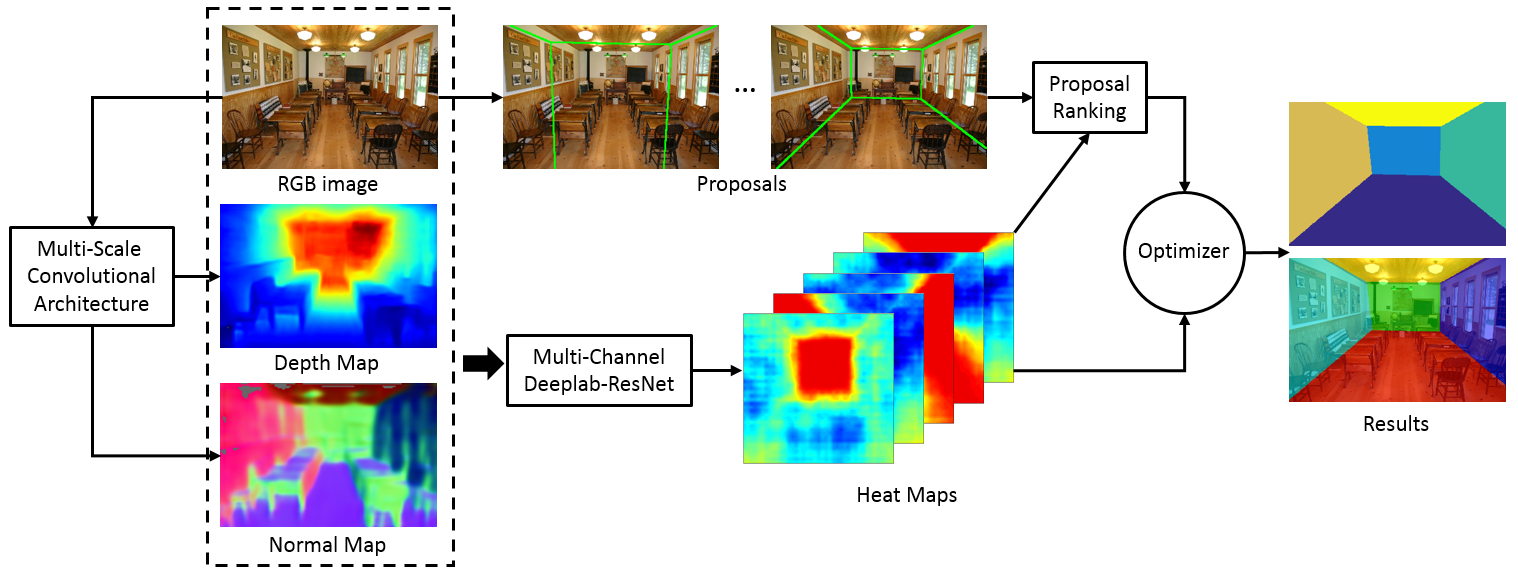
\includegraphics[width=8.5cm]{figure/ppline.png}
	\caption{The pipeline of our layout estimation algorithm. First we adopt a multi-scale CNN achitecture \cite{eigen2015predicting} to extract geometric information from RGB images, including depth and normals. Then we combine all the abovementioned information into a multi-channel FCN , which helps to accurately estimate the layout. Finally, an optimization framwork is employed to obtain final precise layout by optimizing the best proposals generated from RGB images.}
	\label{fig:pipeline}
\end{figure}

Under the Manhattan world assumption, a room layout can be represented as a cube having at most five surfaces \{Left, Front, Right, Ceiling, Ground\} visible in an image. 
%
Given an RGB image $\vb{I}$ with arbitrary size, our algorithm generates a room layout $\vb{L}$ that has a surface label for each pixel $L_{ij} $ in such 5-class set. Fig. \ref{fig:pipeline} shows our algorithm pipeline. 
%%step 1
Different from \cite{dasgupta2016delay,ren2016coarse}, we first estimate depth map $D_{I}$ and normal map $N_{I}$ from the input image to generate geometric hints using a multi-scale convolutional architecture~\cite{eigen2015predicting}, as described in Sec.~\ref{sec:depth_normal}.
%step 2
After that, to integrate information from the original RGB image together with the geometric hints, a multi-channel fully convolutional network(MC-FCN) is trained. The MC-FCN is applied to predict five probability maps, each of which describes the belief for a specific layout surface, see details in Sec.~\ref{sec:surfacelabel}.
%step 3: optimization
While we can easily get access to a layout estimation $\vb{\hat{L}}$ by just choosing the label with the highest score across five probability maps for each pixel. 
The estimated $\vb{\hat{L}}$ always have wavy boundaries and multiple disjoint connected domains due to the characteristics of neural network, see Fig.~\ref{fig:qualitative}. To handle these problems and obtain more clear layout estimation with geometric constraints, an optimization step is adopted in Sec.~\ref{sec:optimization}.  
 

\subsection{Geometric Hints Extraction}
\label{sec:depth_normal}

We use the multi-scale convolutional network proposed in \cite{eigen2015predicting} to estimate the depth and normal maps from RGB images, some qualitative results are shown in Figure~\ref{fig:depthandnormal}. Note that we do not finetune their models with our data as we do not have the depth and normals of our dataset, however, the model seems to generalize well in our case. Quantitive evaluation of their work can be refered to in ~\cite{eigen2015predicting}.
%

\begin{figure}
	\centering
	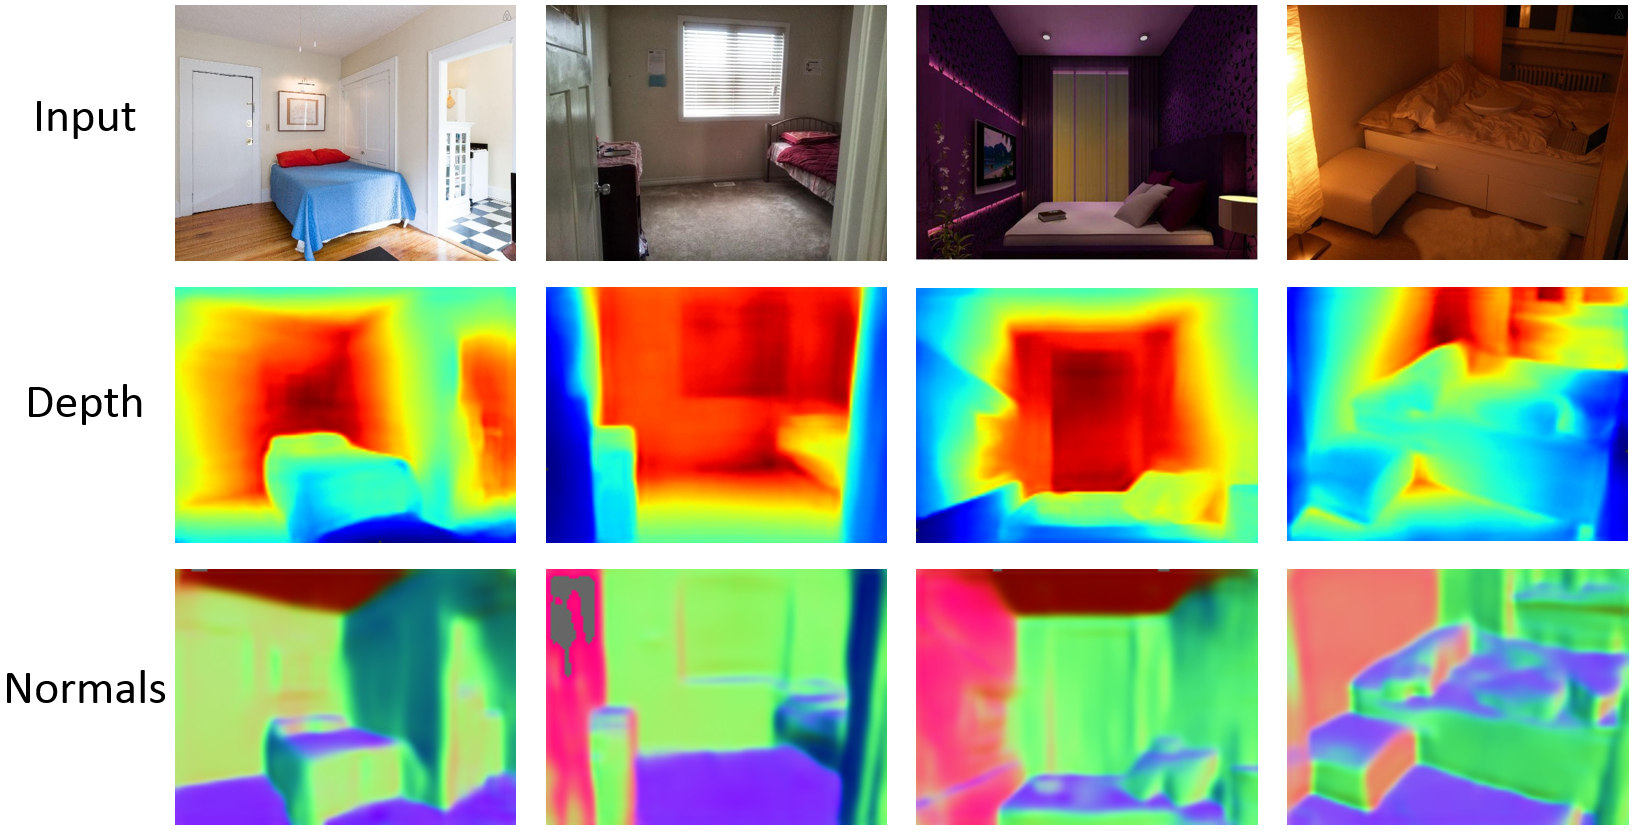
\includegraphics[width=8.5cm]{figure/extractDN.png}
	\caption{Depth and normals estimated from RGB images using the multi-scale FCN in \cite{eigen2015predicting} without finetune. From the global perspective, these geometric information can capture the overall spatial relationships between semantic surfaces. }
	\label{fig:depthandnormal}
\end{figure}

We notice in practice that the depth and normals estimated from RGB images are not precise in local details. And the output resolution of the depth and normal maps are limited to half of the input. However, the valuable 3D information they provide is much helpful for high-level structure estimation, especially in messy scenes.  
%
As depicted in Fig.~\ref{fig:fcn-comparison}, depth and normals can serve as hints tending to merge big planes together under the interference factors like clutter and occlusion. 
%
Therefore, we can apply these mid-level geometric hints to improve the performance of layout estimation. 
%


The depth maps are color coded to 3-channels in \cite{eigen2015predicting} for distinction. In order to ensure the essence of depth and to reduce the redundant information, we modify their rendering section to obtain depth maps with single channel.

\subsection{Semantic Surface Segmentation Using MC-FCN}
\label{sec:surfacelabel}
In some previous works, FCNs are used for semantic surface segmentation \cite{dasgupta2016delay,ren2016coarse,mallya2015learning}. 
%
However, due to clutter, occlusion, complex textures and illumination variations in indoor scenes, the surface segmentation represented as $\vb{\hat{L}}$ are sometimes ruined by irregular spurious regions. Fig.~\ref{fig:fcn-comparison} demonstrates several typical bad cases.
%
To get rid of these annoying spurious regions, we attempt to make our network more robust to miscellaneous environmental factors. And for this purpose, a multi-channel FCN(MF-FCN) is adopted to incorporate geometric hints generated from the original image. 
%

\comments{
The comparison between the predicted results and the ground truth reveals that due to the complex environmental factors of indoor scenes, layout results estimated from FCNN are not very reliable sometimes. 
When the occlusion happens to be at the boundaries of semantic planes, such critical clues are partially or entirely excluded, and thus we can not tell location of each plane precisely. 
Moreover, an entire plane may be predicted separately into pieces due to clutter lay in the plane.}


\begin{figure}
	\centering
	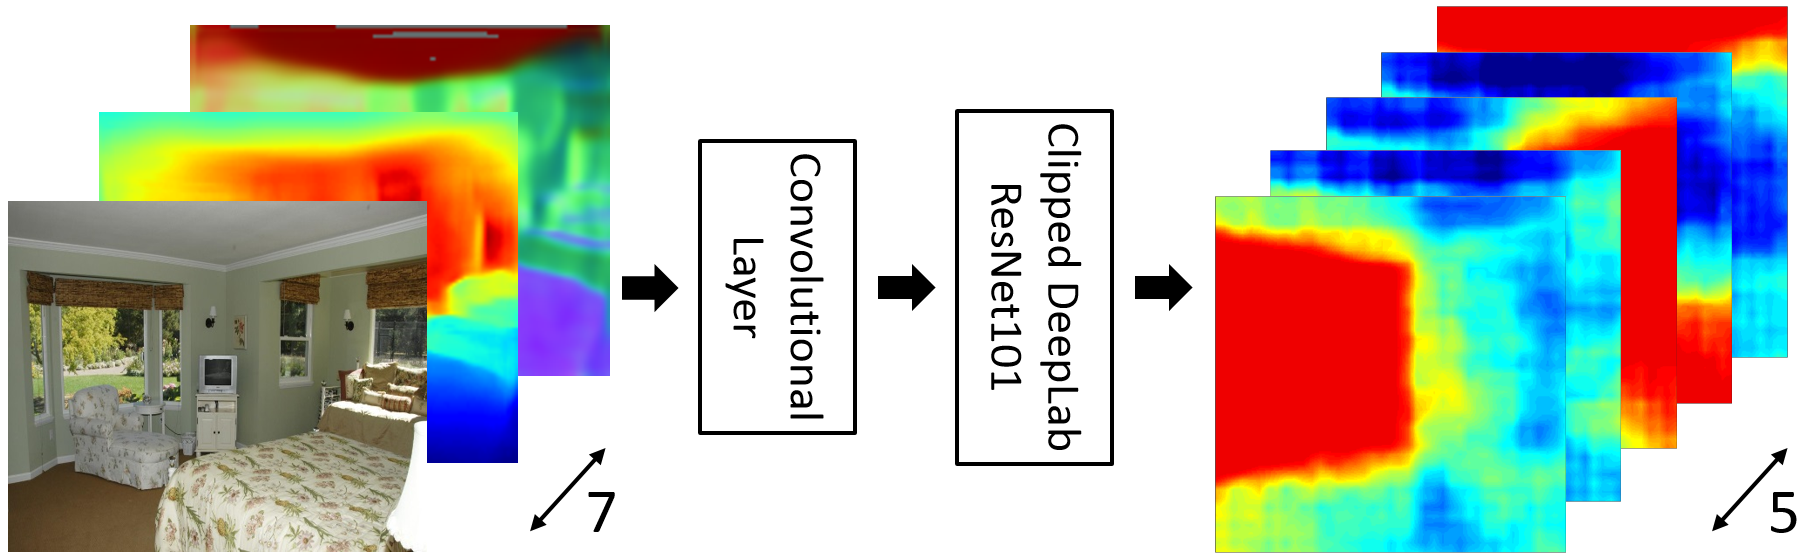
\includegraphics[width=8.5cm]{figure/MC-FCN.png}
	\caption{Illustration of the multi-channel network architecture build on \cite{chen2016deeplab}. We clip the Deeplab-ResNet101 by removing the multi-scale related layers. Then we combine the RGB image, depth and normals together as input to the network for semantic surface learning. }
	\label{fig:fcn-multi-channel}
\end{figure}


\textbf{Network Architecture}
We build the MC-FCN on a famous architecture ResNet-101 \cite{he2016deep} modified by \cite{chen2016deeplab}. As illustrated in Fig.~\ref{fig:fcn-multi-channel}, the estimated depth and normal maps are treated as additional channels associated with the input RGB images. The DeepLab-ResNet101 in \cite{chen2016deeplab} is designed to be multi-scale for semantic segmentation. While we consider the room layout as a high-level semantic information which is more dependent on global information, we further modify the network by clipping the multi-scale related layers. 

\textbf{Training}
We simply concatenate different types of data to a seven-channels input(3 channels from RGB, 1 channel from depth and 3 channels from normals) which is then fed into our network. The model we used for initialization from \cite{chen2016deeplab} is pretrained on MS-COCO dataset. We randomly initialize the weights for the first convolution layer to adapt to our input format. The original classifier layer is replaced with a randomly initialized 5-way classifier layer. Then we specifically finetune our MC-FCN for semantic surface segmentation. We have also tried multi-task learning by adding a new branch for learning boundaries among surfaces as \cite{ren2016coarse, mallya2015learning} do. But the joint training does not help to improve the performance of both tasks in our case. This may indicate that our geometric hints have already integrated the additional information which should be learned through joint training.

The output of our MC-FCN is a $w\times h \times 5$ probability array $\vb{T}$, where $w$ and $h$ stand for the width and length of the input image. Each of the 5 slices can be viewd as a probability map for the corresponding surface label, see Fig.~\ref{fig:fcn-multi-channel}. We utilize the probability array $\vb{T}$ as the basis for our scoring function in both proposals ranking and optimization step. 

\comments{Then an optimization step based on this score function is applied to obtain precise layout estimation.}
\comments{Some visualized results compared with FCN without geometric hints as additional input are shown in Fig.~\ref{fig:fcn-comparison}.}

\subsection{Layout Optimization}
\label{sec:optimization}
We adopt a popular model that several researchers ~\cite{hedau2009recovering, wang2013discriminative, dasgupta2016delay, ren2016coarse} have used to parameterize indoor layout based on the Manhattan world assumption. 
Indoor scene layout is modeled as the projection of a cuboid which can be defined by 

\begin{equation}
	\label{eq:Layout}
	\tau = (l_1, l_2, l_3, l_4, vp_3)
\end{equation}

\begin{figure}
	\centering
	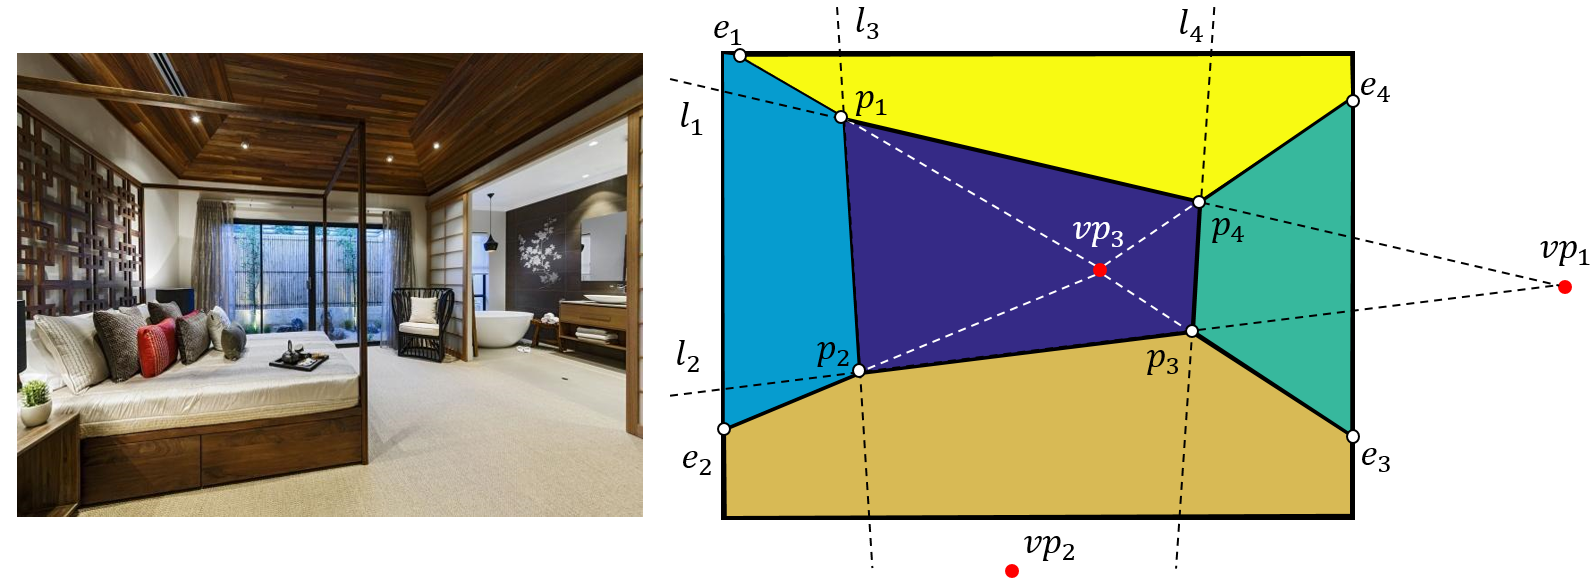
\includegraphics[width=8.5cm]{figure/parameterization.png}
	\caption{(a) Ambiguity between front wall and right/left wall. (b) Illustration of the parameterized model $\tau$. }
	\label{fig:parameterization}
\end{figure}
where $l_{i}$ stands for the $i^{th}$ line and $v$ stands for the vanishing point near the image center, as illustrated in Fig.~\ref{fig:parameterization}(b).
%
Dasgupta et al.~\cite{dasgupta2016delay} propose an iterative refinement algorithm to obtain precise $\vb{L}$. They directly take $\vb{\hat{L}}$ as initialization and preprocess it to address spurious regions and multiple disjoint components. However, as mentioned above, the initial $\vb{\hat{L}}$ generated from $\vb{T}$ are sometimes too ambiguous due to the characteristics of neural networks. The preprocessing step can not adapt to all the misleading situations, especially when the size of ambiguous walls are close. 
%%
\comments{
The whole scene is equivalent to be labeled with five semantic surfaces, coresponding to \{Left, Front, Right, Ceiling, Ground\}, as described in Fig. \ref{fig:2.model}. Based on Eq. (\ref{eq:Layout}), each surface can be reconstructed with extension lines between vanishing point $v$ and Intersection point $p_i$ among $l_{i}$. ie $ve_i$ . Due to the uncertainty of camera pose, five surfaces are not always visible. Examples with different topologies are given in Fig. \ref{fig:different-layout-type}.
%%
To obtain the optimized box layout $\vb{L}$, \cite{dasgupta2016delay} has propose a refinement algorithm. They first generate an initial $\vb{\hat{L}}$ by pick the label with the highest score across five channels of $\vb{T}$. Then a preprocessing step is used to address spurious regions and multiple disjoint components in $\vb{\hat{L}}$. Finally, an iterative optimization method is employed to acquire the refined $\vb{L}$. However, the initial $\vb{\hat{L}}$ generated from $\vb{T}$ are sometimes too ambiguous due to the characteristics of neural network. The preprocessing step can't adapt to all the bad situations well, especially when the ambiguous walls are close in size. 
}

To make the optimization method more general and efficient, we simplify the refinement algorithm in \cite{dasgupta2016delay} by replacing the initialization and preprocessing step with a proposing-ranking framework. The  framework directly generates the initial $\vb{L^*}$ consistent with the formulation in Eq.~\ref{eq:Layout}. This kind of $\vb{L^*}$ is much robust to ambiguous cases and easier for the optimization step to find the best layout.

Our proposing-ranking framework is implemented using the proposing approach in \cite{hedau2009recovering} and constructing a score function based on $\vb{T}$. First, We sample 30 rays from $vp_1$ and $vp_2$ separately to acquire numerous proposals. Then, for any given proposal $\vb{\overline{L}}$ with $r$ semantic surfaces, we define the score function:
%
\begin{equation}
\label{eq:scorefunction}
S(\vb{\overline{L}}~|~\vb{T}) = \frac{1}{wh}\sum_r \vb{T}_r^{(\overline{L}_r)}
\end{equation}
%
Where the subscript $r$ represents a certain region for the corresponding semantic surface. Then we select the proposal with the highest score as initial $\vb{L^*}$, namely:
%
\begin{equation}
\label{eq:initial}
\vb{L^*} = \arg\max_{\overline{L}} S(\vb{\overline{L}}~|~\vb{T})
\end{equation}
%
We further modify the score function and apply it to the following optimization step:
%
\begin{equation}
\label{eq:optimize}
S(\vb{L}~|~\vb{T}) = \frac{1}{wh}\sum_{r} \vb{T}_{r}^{L_{r}} + \frac{1}{wh}\sum_{r^*} \arg\max_{L_{r^*}} \vb{T}_{r^*}^{L_{r^*}}
\end{equation}
%
Where $r \in$ \{Ceiling, Floor\} and $r^* \in$ \{Left, Front, Right\}. The second term including an argmax operation is designed for three walls. As shown in Fig.~\ref{fig:parameterization}(a), there is an inherent ambiguity between front wall and right/left wall. While Dasgupta et al. \cite{dasgupta2016delay} treat it as a special case, our score function cope with the ambiguity generally.

\comments{
	First, We sample 30 rays from $vp_1$ and $vp_2$ separately to acquire numerous proposals. Then, we extend the modified score function in \cite{dasgupta2016delay} for special cases to adapt to all images. Given a specific label, We simply sum up the probability across 5 channels of $\vb{T}$ separately in the same region and choose the maximum as the score for this specific label. This policy is applied just among three walls which mainly cause the ambiguity. The same extended score function is adopted in optimization step. Our postprocessing framework generalize well to ambiguous cases.
}
